\section{Tài nguyên}

\subsection{Bộ dữ liệu}
Bài viết sử dụng 3 bộ dữ liệu lấy từ dữ liệu chất lượng không khí trên trang web aqicn.org từ 01/03/2019 - 01/06/2024 ở 3 thành phố Hà Nội, Hạ Long và Việt Trì. Bộ dữ liệu bao gồm các thuộc tính cụ thể sau:
\begin{table}[h]
  \centering
  \caption{Mô tả thuộc tính}
  \begin{tabular}{|c|c|}
    \hline
    \textbf{Thuộc tính} & \textbf{Mô tả} \\ \hline
    Ngày & Thời gian (YYYY-MM-DD) \\ \hline
    Pm25 & Bụi mịn có đường kính từ 2.5 đến 10 micron \\ \hline
    Pm10 & Bụi mịn có đường kính nhỏ hơn 2.5 micron \\ \hline
    O3 & Ozon \\ \hline
    NO2 & Đioxit nitơ \\ \hline
    SO2 & Đioxit lưu huỳnh \\ \hline
    CO & Carbon monoxit \\ \hline
  \end{tabular}
\end{table}

\begin{table}[h!]
\centering
\caption{Thống kê mô tả cho Hạ Long, Hà Nội và Việt Trì}
\label{tab:stats}
\begin{tabular}{|c|c|c|c|}
\hline
\textbf{Thống kê} & \textbf{Hạ Long} & \textbf{Hà Nội} & \textbf{Việt Trì} \\
\hline
Count & 1920 & 1920 & 1920 \\
Mean & 40.08 & 63.09 & 42.39 \\
Std Dev & 22.95 & 40.26 & 31.66 \\
Min & 5 & 2 & 1 \\
Q1 & 22 & 31 & 19 \\
Q2 (Median) & 38 & 54.5 & 35 \\
Q3 & 54 & 88 & 59 \\
Max & 163 & 217 & 178 \\
Mode & 5 & 24 & 1 \\
Variance & 527.01 & 1620.88 & 1002.69 \\
Kurtosis & 0.41 & 0.334 & 1.92 \\
Skewness & 0.685 & 0.902 & 1.24 \\
CV & 0.572 & 0.638 & 0.74 \\
\hline
\end{tabular}
\end{table}


\begin{figure}[H]
  \centering
  \begin{minipage}{0.15\textwidth}
  \centering
  \end{minipage}
  \hfill

  \begin{minipage}{0.15\textwidth}
      \centering
      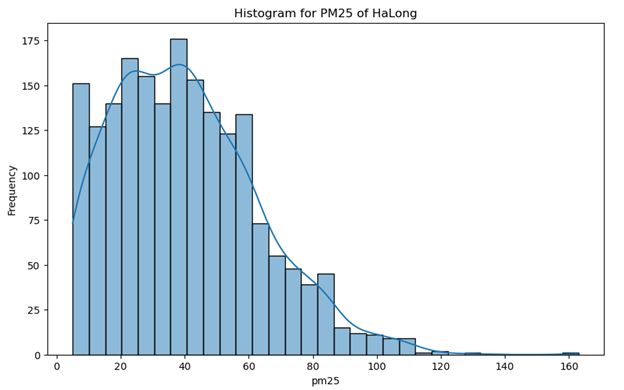
\includegraphics[width=1\textwidth]{img/final/Dataset/histogram.png}
      \end{minipage}
      \hfill
      \begin{minipage}{0.15\textwidth}
      \centering
      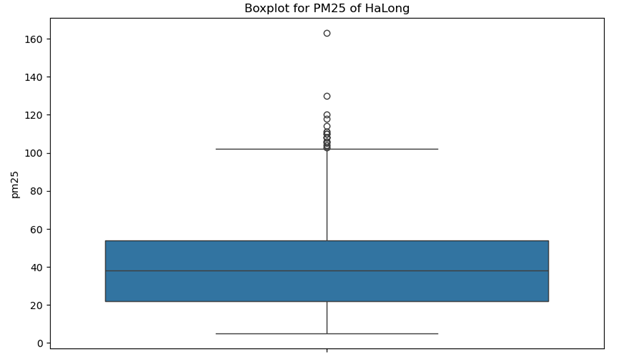
\includegraphics[width=1\textwidth]{img/final/Dataset/boxplot.png}
      \end{minipage}
      \hfill
      \begin{minipage}{0.15\textwidth}
      \centering
      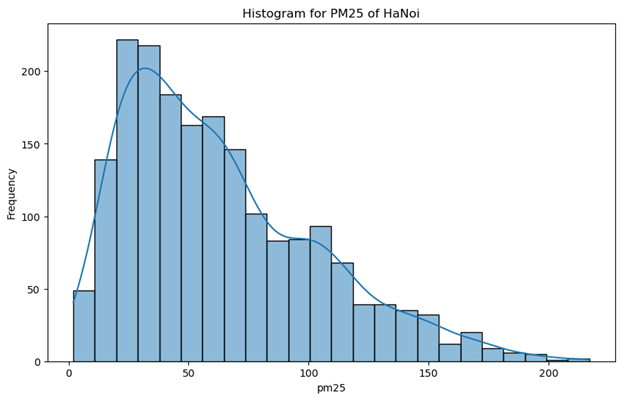
\includegraphics[width=1\textwidth]{img/final/Dataset/histogram_hn.png}
      \end{minipage}
      \hfill

  \begin{minipage}{0.15\textwidth}
      \centering
      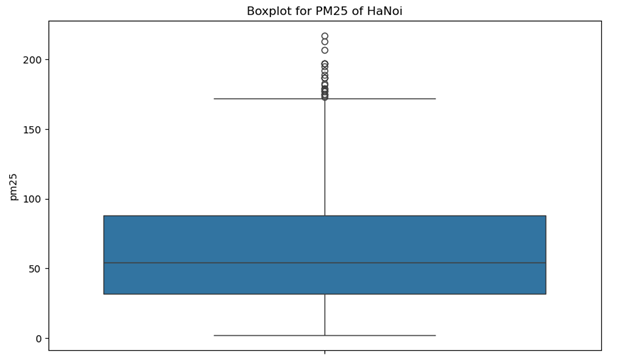
\includegraphics[width=1\textwidth]{img/final/Dataset/boxplot_hn.png}
      \end{minipage}
      \hfill
      \begin{minipage}{0.15\textwidth}
      \centering
      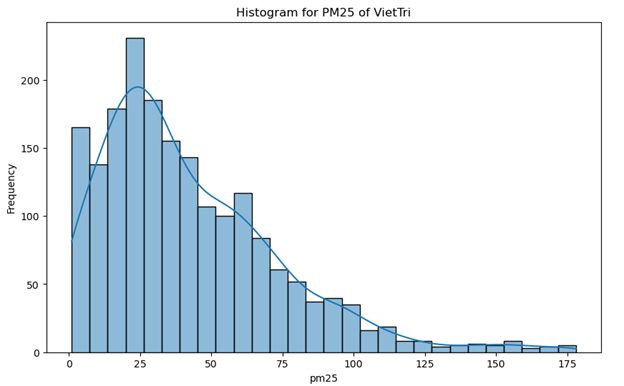
\includegraphics[width=1\textwidth]{img/final/Dataset/histogram_vt.png}
      \end{minipage}
      \hfill
      \begin{minipage}{0.15\textwidth}
      \centering
      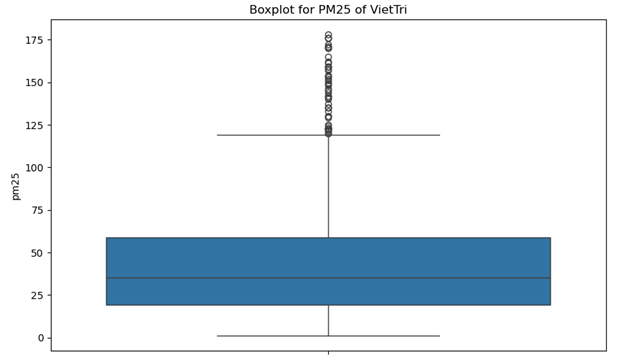
\includegraphics[width=1\textwidth]{img/final/Dataset/boxplot_vt.png}
      
      \end{minipage}
      \hfill
  
  \caption{Biểu đồ histogram và boxplot}
  \label{fig:Random_Forest}
\end{figure}

Dựa vào bảng thống kê mô tả cho Hạ Long, Hà Nội và Việt Trì, chúng ta có thể rút ra các nhận xét sau:

\textbf{Trung bình:} Hà Nội có giá trị trung bình cao nhất (63.09), tiếp theo là Việt Trì (42.39) và Hạ Long (40.08).

\textbf{Độ lệch chuẩn:} Hà Nội có độ lệch chuẩn cao nhất (40.26), cho thấy mức độ biến động lớn hơn so với Hạ Long (22.95) và Việt Trì (31.66).

\textbf{Phân vị:} Các giá trị phân vị (Q1, Q2, Q3) của Hà Nội đều cao hơn so với Hạ Long và Việt Trì, phản ánh sự phân phối dữ liệu cao hơn.

\textbf{Giá trị cực đại:} Hà Nội có giá trị cực đại cao nhất (217), trong khi Hạ Long và Việt Trì lần lượt là 163 và 178.

\textbf{Phương sai:} Hà Nội có phương sai lớn nhất (1620.88), tiếp theo là Việt Trì (1002.69) và Hạ Long (527.01).

\textbf{Độ nhọn và Độ lệch:} Việt Trì có độ nhọn (1.92) và độ lệch (1.24) cao nhất, cho thấy phân phối dữ liệu lệch về phía phải và có đỉnh cao hơn.

\textbf{Hệ số biến thiên (CV):} Việt Trì có hệ số biến thiên cao nhất (0.74), chỉ ra mức độ biến động dữ liệu lớn hơn so với Hà Nội (0.638) và Hạ Long (0.572).

\textbf{Tổng quan:} Hà Nội có giá trị trung bình cao nhất nhưng mức độ biến động và phân tán cũng lớn nhất, thể hiện sự đa dạng trong các giá trị đo lường. Việt Trì có sự biến động và phân tán dữ liệu khá cao, trong khi Hạ Long có dữ liệu ổn định hơn.


\subsection{Công cụ}
Trong quá trình nghiên cứu và phân tích dữ liệu, Nhóm đã tận dụng một loạt các công cụ phân tích thống kê trong Python để khám phá sâu hơn các mẫu dữ liệu và rút ra những kết luận có ý nghĩa. Các công cụ chính bao gồm: Darts, numpy, pandas, sklearn, matplotlib.pyplot,... Sử dụng các công cụ phân tích thống kê này đã giúp Nhóm em hiểu sâu hơn về dữ liệu và đưa ra dự báo. Chi tiết các kết quả có thể được tìm thấy trong bảng mô tả và biểu đồ đi kèm.

% \subsection{Tỷ lệ phân chia dữ liệu}
% Trong quá trình phân tích dữ liệu chuỗi thời gian, Nhóm em đã chia tập dữ liệu thành hai phần: tập huấn luyện và tập kiểm tra, với các tỷ lệ khác nhau như 70\% cho huấn luyện và 30\% cho kiểm tra, 80\% cho huấn luyện và 20\% cho kiểm tra, và 90\% cho huấn luyện và 10\% cho kiểm tra. Những tỷ lệ này giúp Nhóm đánh giá cách mà chúng ảnh hưởng đến hiệu suất của mô hình bằng cách xem xét sự phân phối của dữ liệu trong mỗi tập. Tỷ lệ phổ biến nhất là 7:3, chia 70\% dữ liệu cho huấn luyện và 30\% cho kiểm tra, tạo ra sự cân bằng giữa việc cung cấp đủ dữ liệu huấn luyện và đảm bảo các tập riêng biệt để điều chỉnh và đánh giá. Một lựa chọn khác là tỷ lệ 8:2, ưa chuộng việc sử dụng 80\% dữ liệu cho huấn luyện, có ích cho các mô hình phức tạp yêu cầu tập dữ liệu huấn luyện lớn hơn. Trong một số trường hợp cụ thể, một cách tiếp cận thận trọng như tỷ lệ 9:1 có thể được ưa chuộng, đặc biệt khi xử lý tập dữ liệu lớn và một mô hình đơn giản. Tỷ lệ này đảm bảo có đủ dữ liệu huấn luyện trong khi vẫn giữ được một tập kiểm tra đáng kể để đánh giá hiệu suất. 
\subsection{Tỷ lệ phân chia dữ liệu}
Trong quá trình phân tích dữ liệu chuỗi thời gian, Nhóm đã chia tập dữ liệu thành hai phần: tập huấn luyện và tập kiểm tra, với các tỷ lệ khác nhau như 70\% cho huấn luyện và 30\% cho kiểm tra, 80\% cho huấn luyện và 20\% cho kiểm tra, và 90\% cho huấn luyện và 10\% cho kiểm tra. Tỷ lệ phổ biến nhất là 7:3, tạo sự cân bằng giữa việc cung cấp đủ dữ liệu huấn luyện và đảm bảo các tập riêng biệt để điều chỉnh và đánh giá. Tỷ lệ 8:2 phù hợp cho các mô hình phức tạp cần nhiều dữ liệu huấn luyện, trong khi tỷ lệ 9:1 được ưa chuộng khi xử lý tập dữ liệu lớn và mô hình đơn giản.

\subsection{Đánh giá mô hình}
Trong việc đánh giá hiệu suất của các mô hình, Nhóm em sử dụng ba chỉ số là Mean Absolute Error (MAE), Mean Absolute Percentage Error (MAPE), và Root Mean Squared Error (RMSE). Thuật toán có giá trị thấp nhất trong ba chỉ số này sẽ cho thấy mức độ chính xác tốt nhất. Dưới đây là các công thức để tính MAE, MAPE và RMSE.
\subsection*{Với các tham số: }
\begin{itemize}
    \item \( n \): Số lượng điểm dữ liệu.
    \item \( y_i \): Giá trị thực tế.
    \item \( \hat{y}_i \): Giá trị dự đoán.
\end{itemize}

\subsection*{MAE (Lỗi tuyệt đối trung bình):}
MAE là trung bình của các giá trị tuyệt đối của sai số giữa giá trị dự đoán và giá trị thực tế. Nó đo lường độ lớn của sai số trung bình và không quan tâm đến hướng của sai số. MAE càng nhỏ, mô hình càng chính xác.
\begin{equation}
\text{MAE} = \frac{1}{n} \sum_{i=1}^{n} \left| y_i - \hat{y}_i \right|
\end{equation}

\subsection*{RMSE (Căn bậc hai của trung bình bình phương sai số):}
RMSE là căn bậc hai của trung bình của các bình phương của sai số giữa giá trị dự đoán và giá trị thực tế. Nó đo lường độ lớn của sai số trung bình và cung cấp một con số tương đối về mức độ sai lệch giữa dự đoán và giá trị thực tế. RMSE càng nhỏ, mô hình càng chính xác.
\begin{equation}
\text{RMSE} = \sqrt{\frac{1}{n} \sum_{i=1}^{n} (y_i - \hat{y}_i)^2}
\end{equation}

\subsection*{MAPE (Lỗi phần trăm tuyệt đối trung bình):}
MAPE là trung bình của tỉ lệ phần trăm của sai số tuyệt đối so với giá trị thực tế. Nó thường được sử dụng để đo lường tỷ lệ phần trăm trung bình của sai số so với giá trị thực tế, cung cấp cái nhìn về mức độ chính xác của mô hình dự đoán. MAPE càng nhỏ, mô hình càng chính xác.
\begin{equation}
\text{MAPE} = \frac{1}{n} \sum_{i=1}^{n} \left| \frac{y_i - \hat{y}_i}{y_i} \right| \times 100
\end{equation}